In sum of sinusoids nethod, we use the following architecture to generate different sinusoidal signal
\begin{figure}[H]
    \centering
    \includegraphics[scale = 0.7]{ss.png}
\end{figure}
where 
\begin{equation*}
    g(t) = \sqrt{2} \cdot \left\{\sum_{n=1}^M 2\,(\cos\beta_n + j sin \beta_n)\cos2\pi f_nt + \sqrt{2} \, (\cos\alpha + j sin \alpha)\cos2\pi f_mt\right\}.
\end{equation*}
We plot the envelope and autocorrelation for different $f_mT$ and $M$. Notice that when plotting 
envelope, we neglect the initial part. The reason is that $f_mt$ is small at the beginning, 
resulting in undesired waveform.
\begin{figure}[H]
    \centering
    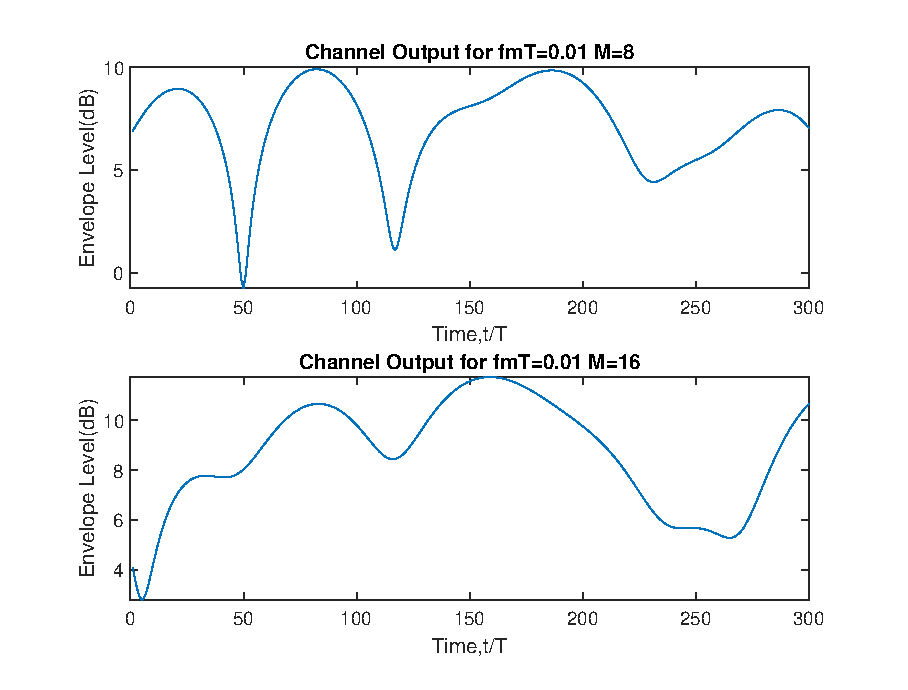
\includegraphics[scale = 0.9]{ss_envelop_001.eps}
\end{figure}
\begin{figure}[H]
    \centering
    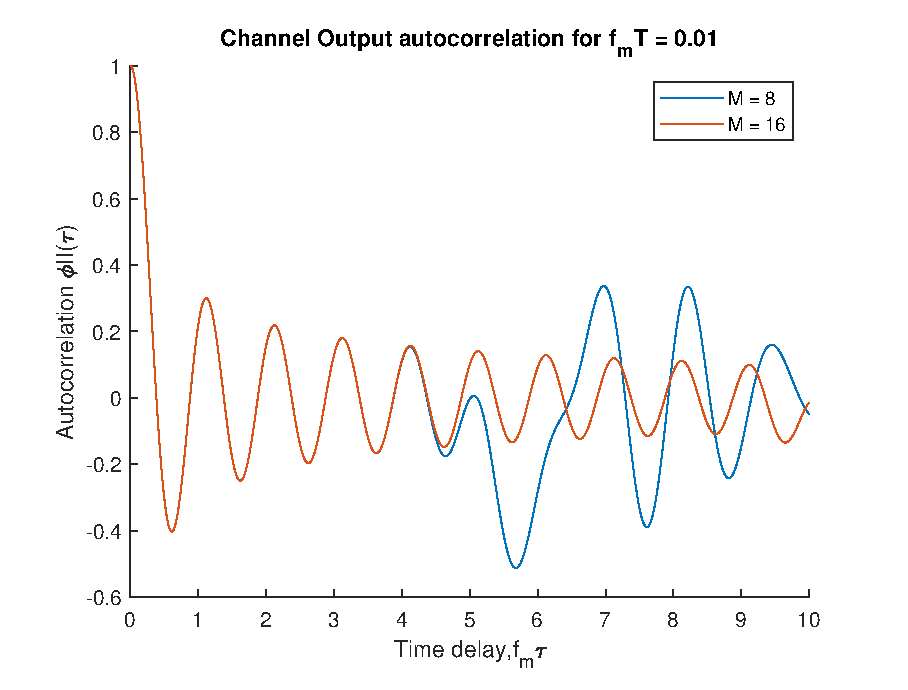
\includegraphics[scale = 0.9]{ss_auto_001.eps}
\end{figure}
\begin{figure}[H]
    \centering
    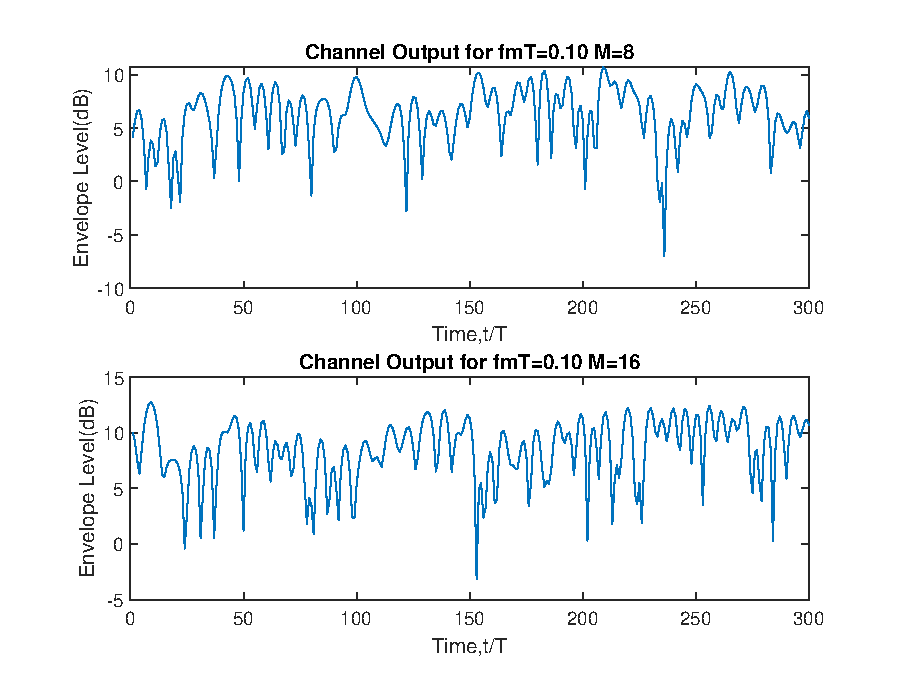
\includegraphics[scale = 0.9]{ss_envelop_01.eps}
\end{figure}
\begin{figure}[H]
    \centering
    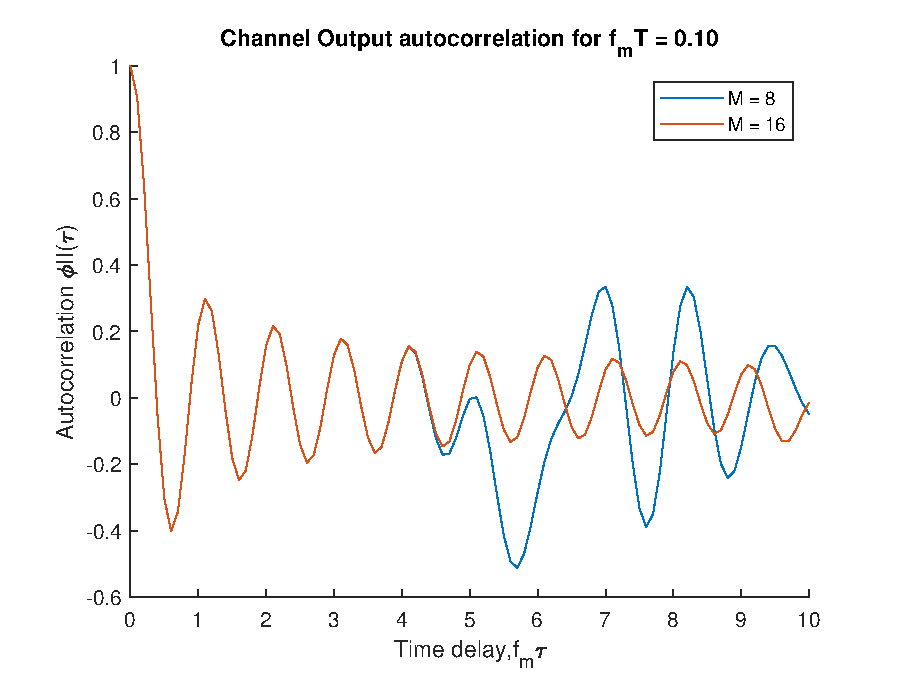
\includegraphics[scale = 0.9]{ss_auto_01.eps}
\end{figure}
\begin{figure}[H]
    \centering
    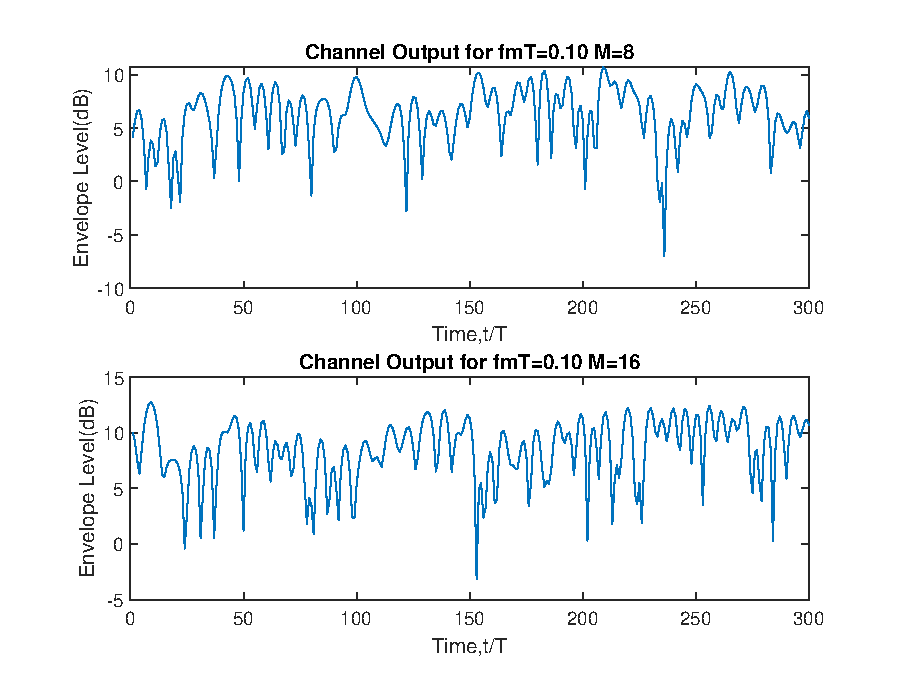
\includegraphics[scale = 0.9]{ss_envelop_01.eps}
\end{figure}
\begin{figure}[H]
    \centering
    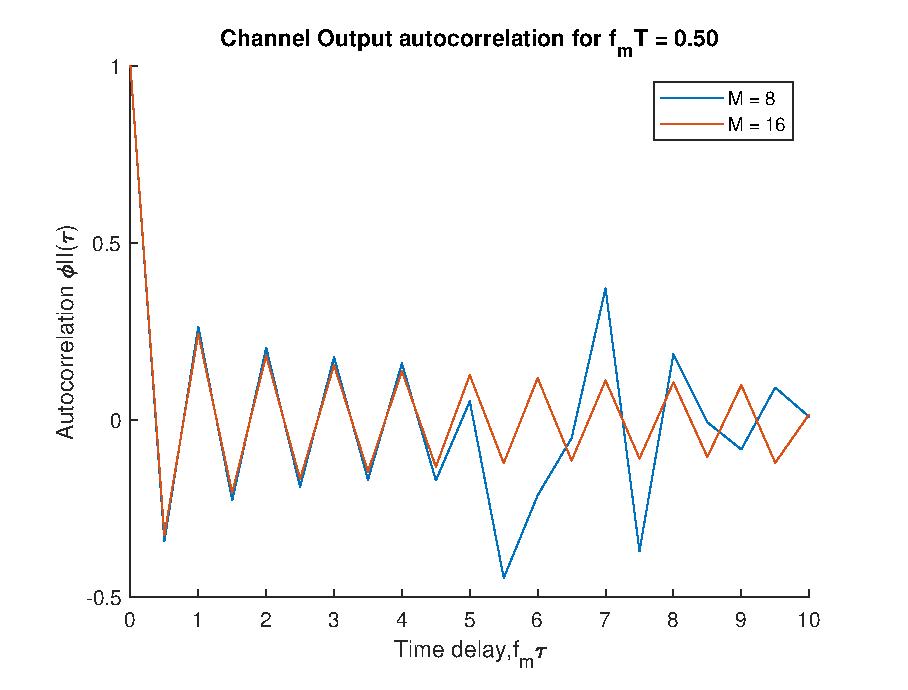
\includegraphics[scale = 0.9]{ss_auto_05.eps}
\end{figure}